\documentclass[final]{beamer}
\usetheme{databrary}
\usepackage[orientation=landscape,size=a0,scale=1.4,debug]{beamerposter}
\usepackage[absolute,overlay]{textpos}
\usepackage{graphics}

\setlength{\TPHorizModule}{1cm}
\setlength{\TPVertModule}{1cm}

\title{Sharing displays and data from vision science research with Databrary}
\author{R.O. Gilmore, K.E. Adolph, D.S. Millman, L. Steiger, and D.A. Simon}
\footer{NSF BCS-1238599, NICHD U01-HD-076595, \& SRCD}
\date{}

\begin{document}
\begin{frame}{} 

\begin{columns}[t]
	\column{.3\textwidth}
		\begin{block}{Motivation}
			The open sharing of data and workflows from scientific research has gained increasing attention in many fields and has become a priority for research funders. 
			Databrary (databrary.org) is a digital data library specialized for storing and sharing video and research data and metadata. Vision scientists often present temporally varying visual displays to human or non-human animal observers and may collect gaze position, kinematic data, or other physiological recordings simultaneously. 
			Some vision scientists collect identifiable video recordings of participants for use in off-line tagging or coding. 
			Databrary may be especially well suited for these use cases because of the library's focus on uploading, organizing, storing, and sharing research data and metadata collected in the course of behavioral resesearch. 
			Databrary has also developed policies that enable identifiable information to be shared with the permission of research participants. 
		\end{block}
		\begin{block}{Privacy \& Security}
			Videos may contain identifiable information such as faces, voices, and images of places. 
			Databrary ensures that identifiable information can be shared in two ways:
			\begin{itemize}
			\item Restricting Access:
				\begin{indent}
					Only those with independent researcher status at an institution may apply for authorization. 
					Applicants promise to uphold ethical principles and sign an access agreement. The institution co-signs the agreement to grant authorization.
				\end{indent}
			\item Securing Permission to Share:
				\begin{indent}
					Identifiable data may only be shared if participants have given informed consent.
					Databrary has developed a release template whose language may be adapted for specific research protocols (https://databrary.org/access/policies.html).
				\end{indent}
			\end{itemize}
		\end{block}
		\begin{block}{What Can Be Shared}
			Databrary can house video, audio, PDF, spreadsheet, image, and text-based files (along with associated metadata), as well as executable scripts in Ruby, R and Matlab that facilitate data analysis.
			Video data are transcoded into standard and HTML5-compatible formats, currently H.264+AAC as MP4. Databrary stores other data in native formats (e.g., .doc, .docx, .xls, .xlsx, .txt, .csv, .pdf, .jpg, .png).
		\end{block}
		\begin{block}{Technology Stack}
			Databary is built on a PostreSQL database using the Scala Play framework and JavaScript.
			Data are preserved indefinitely in a secure data storage facility at NYU managed by the university's central information technologies organization. Central IT staff handle storage, network, and backup systems. NYU does routine tape backups that are stored off site. There is no cost to use the system.
		\end{block}
	\column{.3\textwidth}
		\begin{block}{Databrary.org}
			\begin{center}
				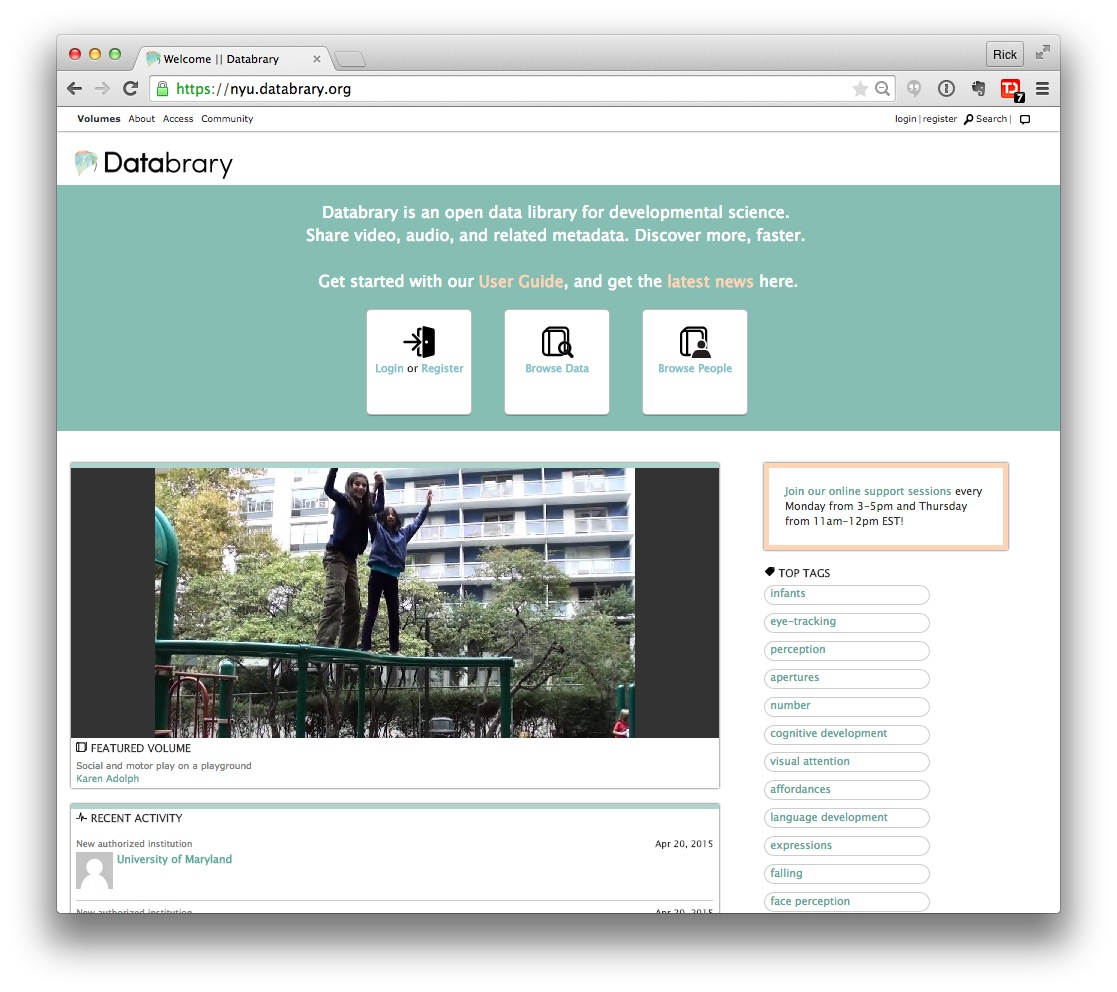
\includegraphics[width=\textwidth]{img/databrary-splash.png}
			\end{center}
			Databrary's splash page shows a feed of recent activity, a set of clickable tags that link to studies with those search terms, a featured dataset, and links that enable users to search for data or manage their own data.
		\end{block}
		\begin{block}{Each Study/Dataset Has Its Own Page}
			\begin{center}
				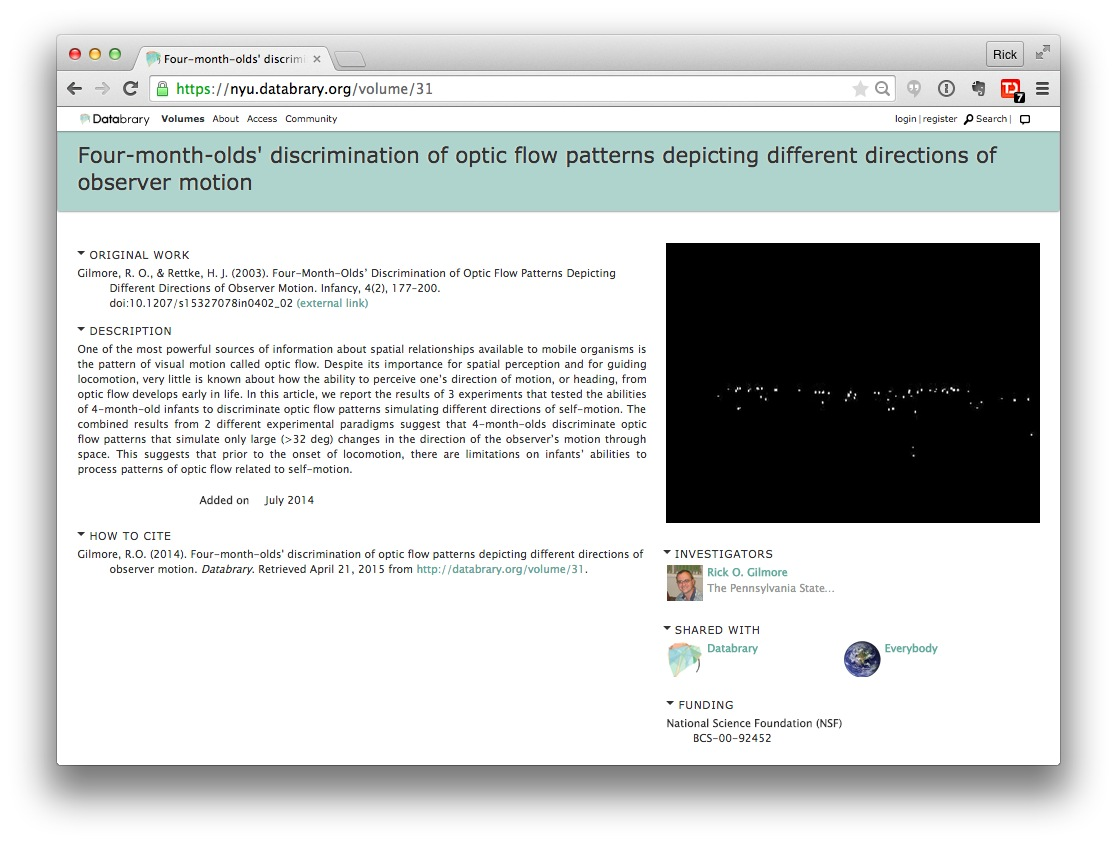
\includegraphics[width=\textwidth]{img/volume-31.png}
			\end{center}
		\end{block}
	\column{.3\textwidth}
		\begin{block}{Data Management for Ongoing Projects}
			\begin{center}
				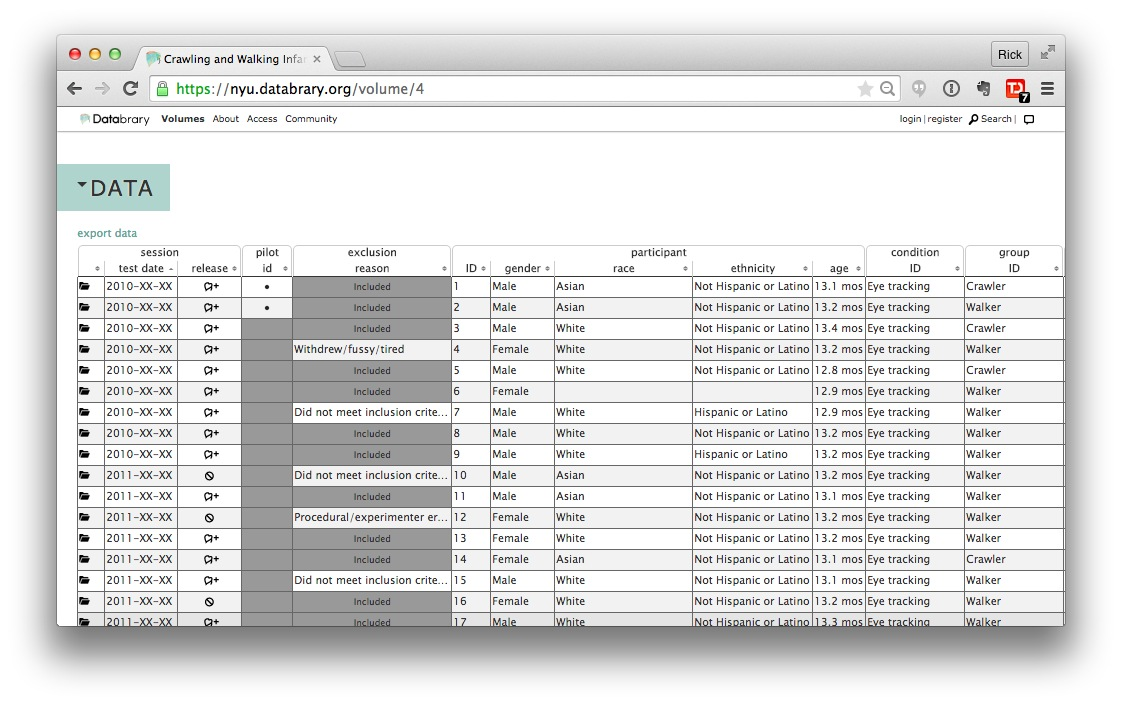
\includegraphics[width=\textwidth]{img/spreadsheet.png}
			\end{center}
			Users may upload video and related data \emph{as they collect it}, recording information about individual data collection sessions such as participant characteristics, sharing permission levels, and study conditions. Once uploaded, the project remains private only to named collaborators until the data owner chooses to share it with Databrary. 
		\end{block}
		\begin{block}{Organize, View. Tag Data in Timeline}
			\begin{center}
				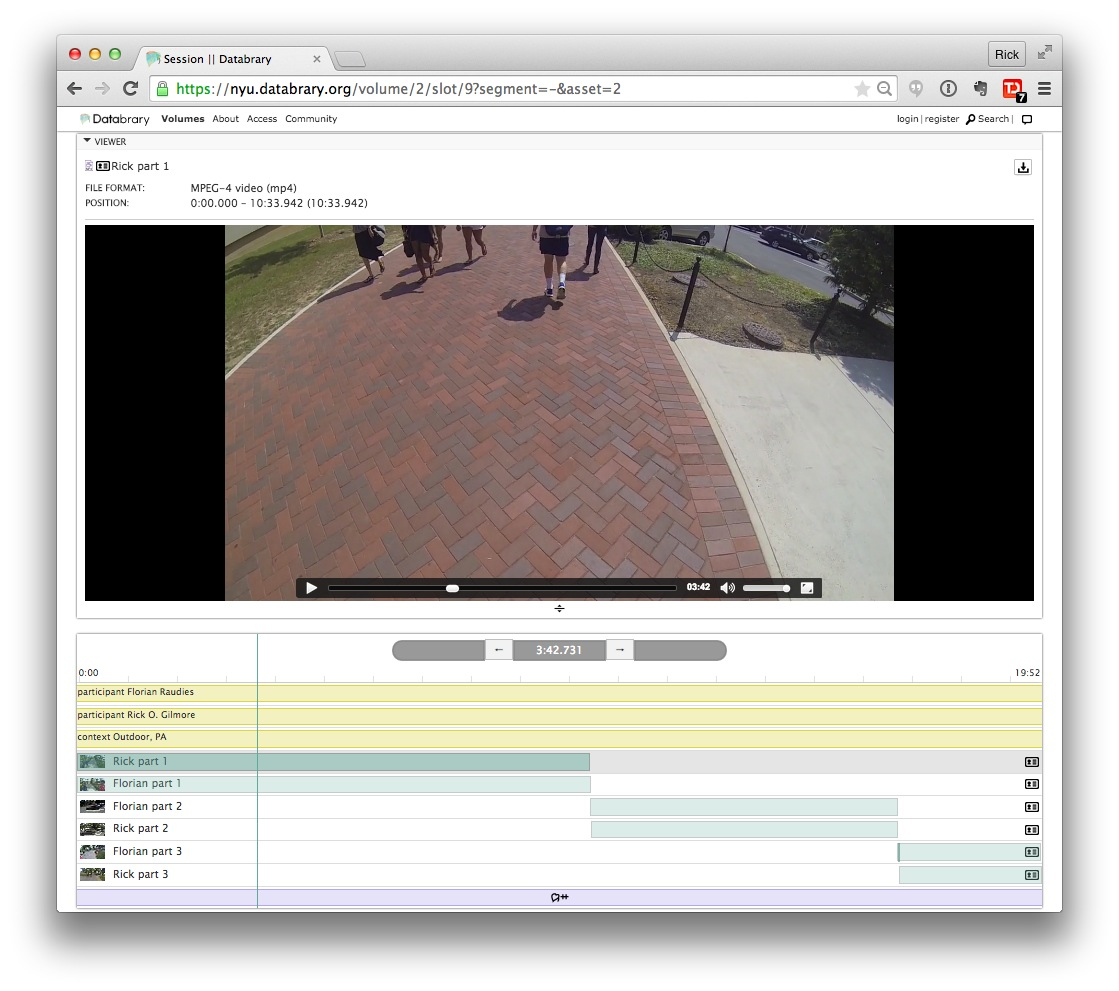
\includegraphics[width=\textwidth]{img/timeline.png}
			\end{center}
			Within a session, data are represented on a timeline that reflects when events occurred. This is particularlly useful for studies with multiple camera views (e.g., eye-tracking) or with combined behavioral and image/display streams.
		\end{block}
\end{columns}

\end{frame}
\end{document}
